\section{Semaine 4 - 26 fev}

\subsection{Lundi}

L'\textbf{objectif} d'aujourd'hui c'est de
\begin{itemize}
    \item Optimiser la bowtie simple
    \item Optimiser la bowtie vraie
    \item Optimiser la dipole
\end{itemize}

Pour les simulations, on a maintenant ajouté une couche d'oxide SiO$_{2}$. C'est cela qu'on voit dans la figure \ref{fig:oxide_film}.

\begin{wrapfigure}{R}{0.4\textwidth}
    \centering
    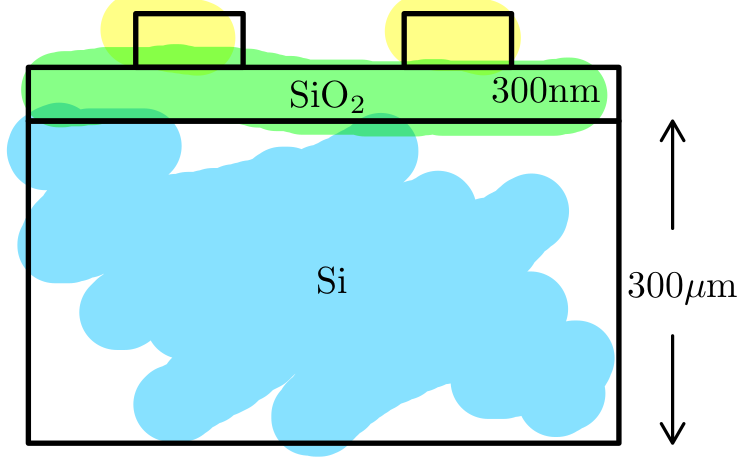
\includegraphics[width=0.35\textwidth]{texfigures/ocide_film.png}
    \caption{\label{fig:oxide_film} On ajoute une couche d'oxide au dessus du substrat.}
\end{wrapfigure}